\documentclass[12pt,letterpaper]{book}
%\documentclass[12pt,letterpaper]{memoir}
% See the ``Memoir customise'' template for some common customisations
% Don't forget to read the Memoir manual: memman.pdf
%% LaTeX - Memoir customise

%% LaTeX Preamble - Common packages
\usepackage[utf8]{inputenc} % Any characters can be typed directly from the keyboard, eg éçñ
\usepackage{textcomp} % provide lots of new symbols
\usepackage{graphicx}  % Add graphics capabilities
%\usepackage{epstopdf} % to include .eps graphics files with pdfLaTeX
\usepackage{flafter}  % Don't place floats before their definition
%\usepackage{topcapt}   % Define \topcation for placing captions above tables (not in gwTeX)
\usepackage{natbib} % use author/date bibliographic citations
\usepackage{color}
%\usepackage{indentfirst} % force to indent at every paragraph

\usepackage{amsmath,amssymb}  % Better maths support & more symbols
\usepackage{bm}  % Define \bm{} to use bold math fonts

\usepackage[pdftex,bookmarks,colorlinks,breaklinks]{hyperref}  % PDF hyperlinks, with coloured links
\definecolor{dullmagenta}{rgb}{0.4,0,0.4}   % #660066
\definecolor{darkblue}{rgb}{0,0,0.4}
\hypersetup{linkcolor=red,citecolor=blue,filecolor=dullmagenta,urlcolor=darkblue} % coloured links
%\hypersetup{linkcolor=black,citecolor=black,filecolor=black,urlcolor=black} % black links, for printed output

\usepackage{memhfixc}  % remove conflict between the memoir class & hyperref
% \usepackage[activate]{pdfcprot}  % Turn on margin kerning (not in gwTeX)
\usepackage{pdfsync}  % enable tex source and pdf output syncronicity

\usepackage{underscore}

%%% PAGE DIMENSIONS
% Set up the paper to be as close as possible to both A4 & letter:
%\settrimmedsize{11in}{210mm}{*} % letter = 11in tall; a4 = 210mm wide
%\setlength{\trimtop}{0pt}
%\setlength{\trimedge}{\stockwidth}
%\addtolength{\trimedge}{-\paperwidth}
%\settypeblocksize{*}{\lxvchars}{1.618} % we want to the text block to have golden proportionals
%\setulmargins{50pt}{*}{*} % 50pt upper margins
%\setlrmargins{*}{*}{1.618} % golden ratio again for left/right margins
%\setheaderspaces{*}{*}{1.618}
%\checkandfixthelayout 
% This is from memman.pdf

%%% \maketitle CUSTOMISATION
% For more than trivial changes, you may as well do it yourself in a titlepage environment
%\pretitle{\begin{center}\sffamily\huge\MakeUppercase}
%\posttitle{\par\end{center}\vskip 0.5em}

%%% ToC APPEARANCE
%\maxtocdepth{subsection} % include subsections
%\renewcommand{\cftchapterpagefont}{}
%\renewcommand{\cftchapterfont}{}     % no bold!

%%% HEADERS & FOOTERS
%\pagestyle{ruled} % try also: empty , plain , headings , ruled , Ruled , companion

%%% CHAPTERS
%\chapterstyle{hangnum} % try also: default , section , hangnum , companion , article, demo

%\renewcommand{\chaptitlefont}{\Huge\sffamily\raggedright} % set sans serif chapter title font
%\renewcommand{\chapnumfont}{\Huge\sffamily\raggedright} % set sans serif chapter number font

%%% SECTIONS
%\hangsecnum % hang the section numbers into the margin to match \chapterstyle{hangnum}
%\maxsecnumdepth{subsection} % number subsections

%\setsecheadstyle{\Large\sffamily\raggedright} % set sans serif section font
%\setsubsecheadstyle{\large\sffamily\raggedright} % set sans serif subsection font

%% END Memoir customise

% Euler for math | Palatino for rm | Helvetica for ss | Courier for tt
\renewcommand{\rmdefault}{ppl} % rm
\linespread{1.05}        % Palatino needs more leading
\usepackage[scaled]{helvet} % ss
\usepackage{courier} % tt
%\usepackage{euler} % math
%\usepackage{eulervm} % a better implementation of the euler package (not in gwTeX)
\normalfont
\usepackage[T1]{fontenc}


%LMH Packages and customizations
\usepackage{bbm} 
\newcommand{\redtext}[1]{\textcolor{red}{[#1]}}  %%% FOR EDITING
%\newcommand{\redtext}[1]{}  %%%FOR RELEASE
\usepackage{lineno}
\usepackage{algorithm}
\usepackage{tcolorbox}
\usepackage{longtable}
\newcommand{\plogo}{\fbox{$\mathcal{PL}$}} % Generic dummy publisher logo

\usepackage[utf8]{inputenc} % Required for inputting international characters
\usepackage[T1]{fontenc} % Output font encoding for international characters
\usepackage{fouriernc} % Use the New Century Schoolbook font
\pagestyle{empty}
%\usepackage{fancyhdr}
%\cfoot{Not for distribution beyond GFDL, GSFC, EMC, CAPS}
%\renewcommand{\headrulewidth}{0.4pt}
%\renewcommand{\footrulewidth}{0.4pt}

%\usepackage[none]{hyphenat}
\newcommand{\fv}{FV$^{\mathrm{3}}$}

%https://tex.stackexchange.com/questions/122119/making-a-title-page-with-a-subtitle-in-memoir
\title{FV$^3$:The GFDL Finite-Volume Cubed-Sphere Dynamical Core}
%\newcommand{\subtitle}{Part I: Scientific description of the dynamical core}
%\title{FV$^3$ : The GFDL Finite-Volume Cubed-Sphere Dynamical Core\\Part I: Scientific description of the dynamical core }
\author{Shian-Jiann Lin, Lucas M. Harris, and William J. Putman\\ \\ with the GFDL \fv\ team}%\redtext{Add names}}
%\date{February 13, 2017}

%\renewcommand{\maketitlehooka}{A}
%\renewcommand{\maketitlehookb}{\centering\textsc{\subtitle}}
%\renewcommand{\maketitlehookc}{C}
%\renewcommand{\maketitlehookd}{D}

%%% BEGIN DOCUMENT
\begin{document}

\begin{titlepage} % Suppresses headers and footers on the title page

	\centering % Centre everything on the title page
	
	\scshape % Use small caps for all text on the title page
	
	\vspace*{\baselineskip} % White space at the top of the page
	
	%------------------------------------------------
	%	Title
	%------------------------------------------------
	
	\rule{\textwidth}{1.6pt}\vspace*{-\baselineskip}\vspace*{2pt} % Thick horizontal rule
	\rule{\textwidth}{0.4pt} % Thin horizontal rule
	
	\vspace{0.75\baselineskip} % Whitespace above the title
	 
	{\LARGE { \huge \fv  } \\  THE GFDL  \\ FINITE-VOLUME CUBED-SPHERE\\ DYNAMICAL CORE\\} % Title
	
	\vspace{0.75\baselineskip} % Whitespace below the title
	
	\rule{\textwidth}{0.4pt}\vspace*{-\baselineskip}\vspace{3.2pt} % Thin horizontal rule
	\rule{\textwidth}{1.6pt} % Thick horizontal rule
	
	\vspace{2\baselineskip} % Whitespace after the title block
	
	%------------------------------------------------
	%	Subtitle
	%------------------------------------------------
	Shian-Jiann Lin, William Putman, Lucas Harris \\
	\vspace{0.75\baselineskip} % Whitespace below the title
	and the GFDL \fv\ team
	\vspace{0.75\baselineskip} % Whitespace below the title
	
 % Subtitle or further description
	
	\vspace*{3\baselineskip} % Whitespace under the subtitle
	
	%------------------------------------------------
	%	Editor(s)
	%------------------------------------------------
	
	%Edited By
	
	\vspace{0.5\baselineskip} % Whitespace before the editors
	
	{\scshape\Large VERSION 1.0 (DRAFT)} % Editor list
	
	\vspace{0.5\baselineskip} % Whitespace below the editor list
	
	\textit{Date \today} % Editor affiliation
	
	\vfill % Whitespace between editor names and publisher logo
	

	
	\vspace{0.3\baselineskip} % Whitespace under the publisher logo
	
	%2017 % Publication year
	
	{\large Responsible Organization: OAR/GFDL} % Publisher

\end{titlepage}

%----------------------------------------------------------------------------------------


\pagebreak

\section*{CHANGE RECORD PAGE}
\begin{center}
    \begin{tabular}{ | p{1.5cm} | p{1.8cm} | l | p{7cm} |}
    \hline
    \textbf{Version} & \textbf{Date} & \textbf{Page affected} & \textbf{Description }\\ \hline
    1.0 (DRAFT) & 11/28/2017 & all & Draft submitted to EMC \\ \hline
%    0.1 & 11/20/2017 & 4, 6-7 & Added a chart at page 4 and edited content from page 6-7  \\ \hline
 %   1.0 & 11/23/2017 &  &  Approved and signed version\\
    \hline
    \end{tabular}
\end{center}

\pagebreak
\newpage

\section*{SIGNATURE PAGE}

\vspace{2.5\baselineskip} % Whitespace before the editors

\indent \indent \indent Prepared by: 

\indent \indent \indent \indent \indent \indent Lucas Harris

\vspace{9.0\baselineskip} % Whitespace before the editors

\indent \indent Approved by: Vijay Tallapragada  

\indent \indent \indent \indent \indent \indent Deputy Director

\indent \indent \indent \indent \indent \indent Date

\vspace{9.0\baselineskip} % Whitespace before the editors

\indent \indent Concurred by: Brian Gross

\indent \indent \indent \indent \indent \indent Acting EMC Director

\indent \indent \indent \indent \indent \indent Date


\eject
\tableofcontents

\chapter*{Disclaimer}

We have made every effort to ensure that the information in this document is as accurate, complete, and as up-to-date as possible. However, due to the rapid pace of \fv\ and \fv-powered model development the document may not always reflect the current state of \fv\ capabilities. Often, the code itself is the best description of the current capabilities and the available options, which due to limited space cannot all be described in full detail here. Contact GFDL FV3 support ( oar.gfdl.fvGFS\_support\@noaa.gov)  for  assistance and more information. 

\chapter{\fv\ introduction}\label{chap:intro}



\section{A brief history of \fv}

\fv\ is a natural evolution of the hydrostatic Finite-Volume dynamical core (FV core) originally developed in the 90s on the latitude-longitude grid. The FV core started its life at NASA/Goddard Space Flight Center (GSFC) during early and mid 90s as an offline transport model with emphasis on the conservation, accuracy, consistency (tracer to tracer correlation), and efficiency of the transport process. The development and applications of monotonicity-preserving Finite-Volume schemes at GSFC were motivated in part by the need to have a solution for the noisy and unphysical negative water vapor and chemical species (L94, LR96). It subsequently has been used by several high-profile Chemistry Transport Models (CTMs), including the NASA-community GMI model (Rotman et al., 2001, J.\ Geophys.\ Res.), GOCART (Chin et al., 2000, J.\ Geophys.\ Res.), and the Harvard University-developed GEOS-CHEM community model (Bey et al, 2001, , J.\ Geophys.\ Res.). This transport module has also been used by some climate models, including the ECHAM5 AGCM (Roeckner et al, 2003, MPI-Report No.\ 349). Motivated by the success of monotonicity-preserving FV schemes in CTM applications, a consistently-formulated shallow-water model was developed. This solver was first presented at the 1994 PDE on the Sphere Workshop, and published in LR97. The Lin-Rood algorithm for shallow-water equations maintains mass conservation and a key Mimetic property of ``no false vorticity generation'', and for the first time in computational geophysical fluid dynamics, uses high-order monotonic advection consistently for momentum and all other prognostic variables, instead of the inconsistent hybrid finite-difference and finite-volume approach used by practically all other ``finite-volume'' models today. The full 3D hydrostatic dynamical core, the FV core, was constructed based on the LR96 transport algorithm and the Lin-Rood shallow-water algorithm (LR97). The pressure gradient force is computed by the L97 finite-volume integration method, derived from Green's integral theorem and based directly on first principles, and demonstrated errors an order of magnitude smaller than other pressure-gradient schemes at the time. The vertical discretization is the ``vertically Lagrangian'' scheme described by L04, the most powerful aspect of \fv, which permits great computational efficiency as well as greater accuracy given the same vertical resolution. The FV core was implemented in the NCAR CESM model in 2001 (Rasch et al, 2006, J.\ Climate) and in the GFDL CM2 model in 2004 (Delworth et al, 2006, J.\ Climate). 

The need to scale to larger number of processors in modern massively-parallel environments and the scientific advantage of eliminating the polar filter led to the development of \fv, the cubed-sphere version of FV. The cubed-sphere \fv\ is in use in all GFDL and GSFC global models, and the cubed-sphere version of the LR96 advection scheme is used by the most recent version of GEOS-CHEM. Most recently, a computationally efficient non-hydrostatic solver has been implemented using a traditional semi-implicit approach for treating the vertically propagating sound waves. A second option for the non-hydrostatic solver, using a Riemann solver to nearly exactly solve for vertical sound-wave propagation, is also available. The Riemann solver is highly accurate and is very efficient if the Courant number for vertical sound wave propagation is small, and so may be very useful for extremely high ($<1$~km) horizontal resolutions. In July 2016 this nonhydrostatic core has been selected for the Next-Generation Global Prediction System (NGGPS), paving the way for the unification of not only weather and climate models but also potentially regional and global models.

\section{Outline of the solver}

\fv\ is the solver that integrates the compressible, adiabatic Euler equations in a weather or climate model. The solver is modular and designed to be called as a largely independent component of a numerical model, consistent with modern standards for model design; however for best results it is recommended that a model using \fv\ as its dynamical core should use the provided application programming interface (API) to invoke the solver as well as to use the provided utility routines consistent with the dynamics, particularly for the initialization, updating the model state by time tendencies from the physics, and for incorporating increments from the data assimilation system. 

\begin{figure}[t] %  figure placement: here, top, bottom, or page
   \centering
   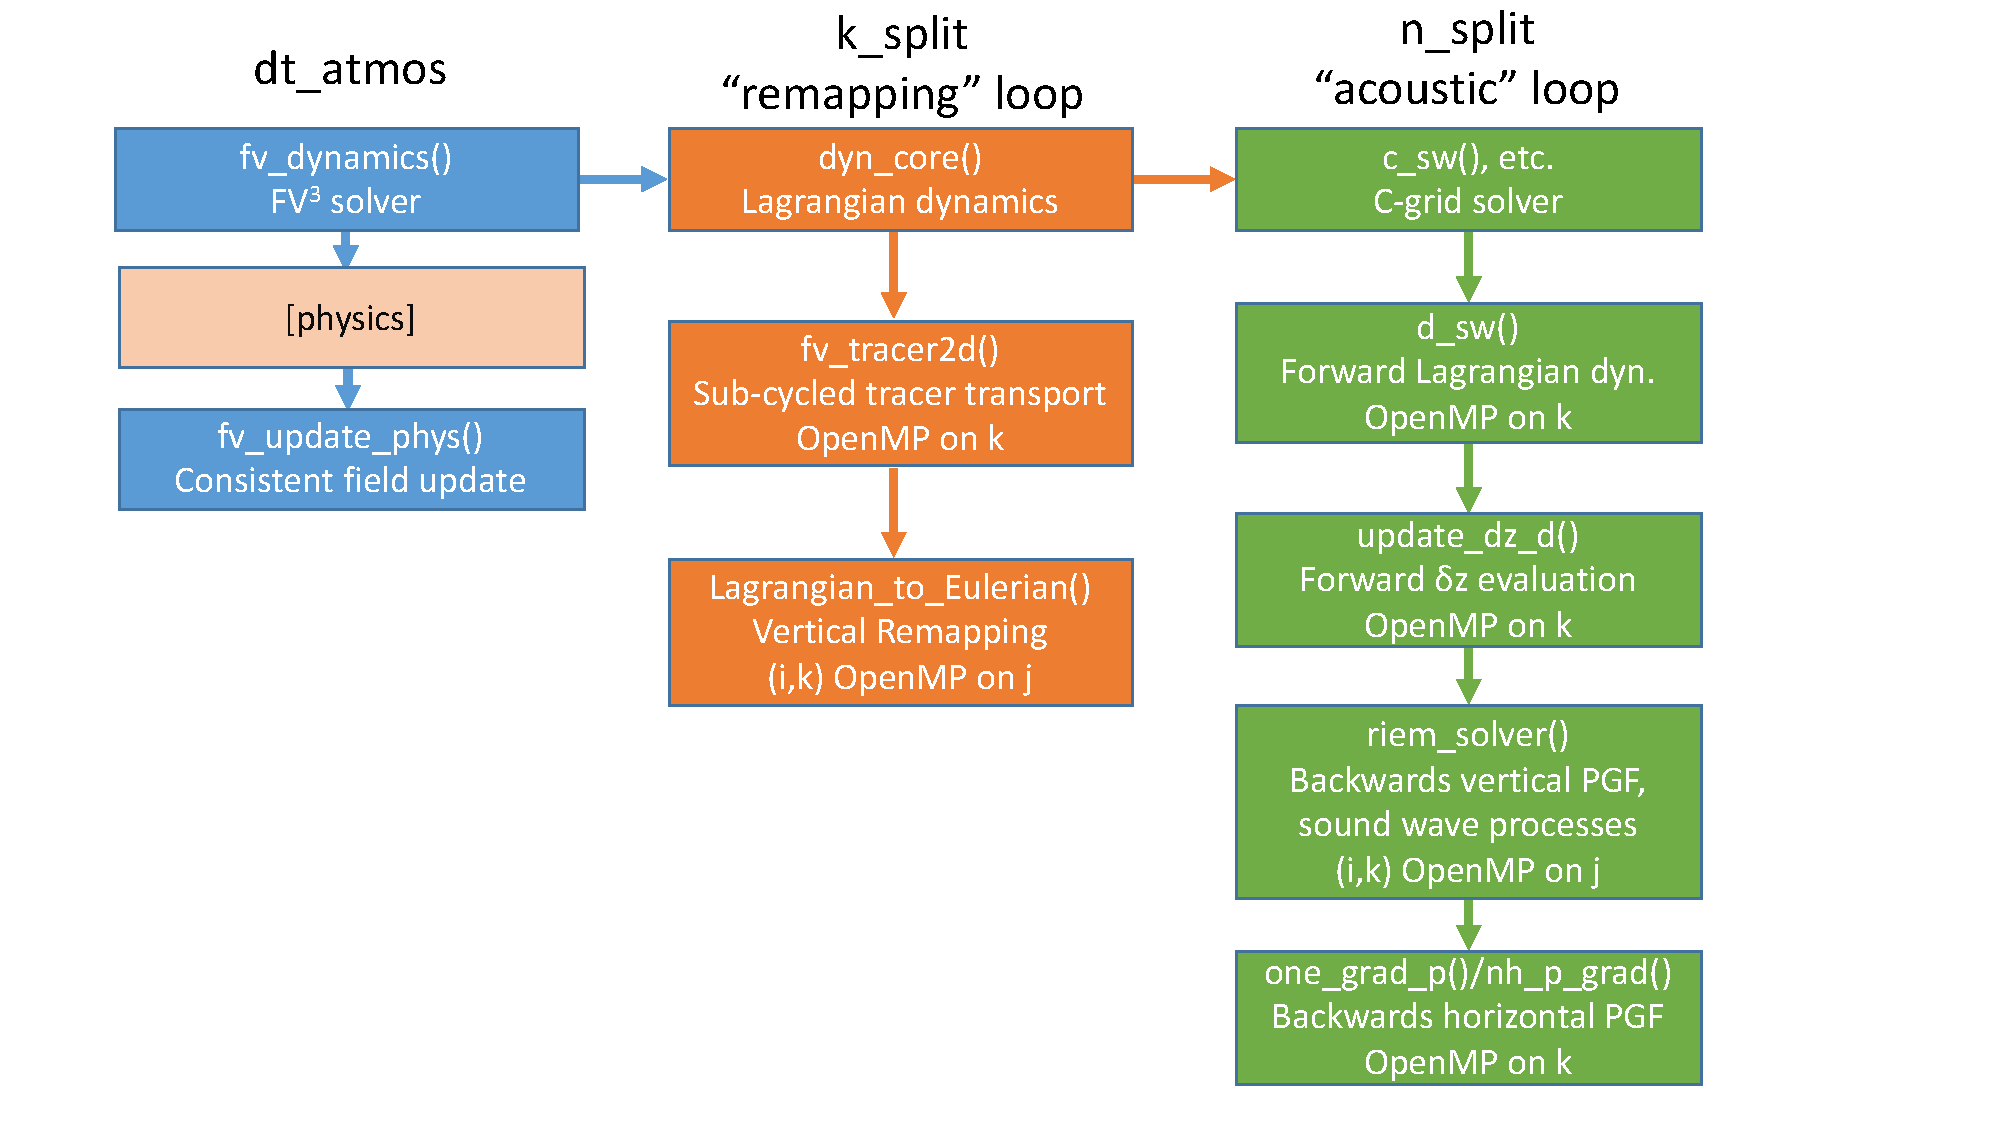
\includegraphics[scale=0.5]{FV3flowchart.pdf} 
   \caption{\fv\ structure, including subroutines and time-stepping. Blue represents external API routines, called once per physics time step; orange routines are called once per remapping time step; green routines once per acoustic time step.}
   \label{fig:flowchart}
\end{figure}


The leftmost column of Figure~\ref{fig:flowchart} shows the external API calls used during a typical process-split model integration procedure. First, the solver is called, which advances the solver a full ``physics'' time step. This updated state is then passed to the physical parameterization package, which then computes the physics tendencies over the same time interval. Finally, the tendencies are then used to update the model state using a forward-in-time evaluation consistent with the dynamics, as described in Chapter~\ref{chap:PDcoupling}.

There are two levels of time-stepping inside \fv. The first is the ``remapping'' loop, the orange column in Figure~\ref{fig:flowchart}. This loop has three steps:
\begin{enumerate}
 \item Perform the Lagrangian dynamics, the loop shown in the green column of Figure~\ref{fig:flowchart}
 \item Perform the sub-cycled tracer advection along Lagrangian surfaces, using accumulated mass fluxes from the Lagrangian dynamics. Subcycling is done independently within each layer to maintain local (within each layer) stability.  %Change from S-J's
 \item Remap the deformed Lagrangian surfaces on to the reference, or ``Eulerian'', coordinate levels. 
\end{enumerate}
This loop is typically performed once per call to the solver, although it is possible to improve the model's stability by executing the loop (and thereby the vertical remapping) multiple times per solver call. 

The Lagrangian dynamics is the second level of time-stepping in \fv. This is the integration of the dynamics along the Lagrangian surfaces, across which there is no mass transport. Since the time step of the Lagrangian dynamics is limited by horizontal sound-wave processes, this is called the ``acoustic'' time step loop. (Note that the typical assumption that the advective wind speed is much slower than the sound wave speed is often violated near the poles, since the speed of the polar night jets can exceed two-thirds of the speed of sound.) The Lagrangian dynamics has two parts: the C-grid winds are advanced a half-time step, using simplified (but similarly constructed) core routines, which are then used to provide the advective fluxes to advance the D-grid prognostic fields a full time step. The integration procedure is similar for both grids: the along-surface flux terms (mass, heat, vertical momentum, and vorticity, and the kinetic energy gradient terms) are evaluated forward-in-time, and the pressure-gradient force and elastic terms are then evaluated backwards-in-time, to achieve enhanced stability. 


\chapter{Stabilization and filtering options} \label{chap:diffusion}

\section{Divergence damping}

Horizontal divergence (along a Lagrangian surface) is computed as a cell-integrated quantity on the dual grid:
\begin{equation}
D = \frac{1}{\Delta A_c} \left [ \delta_x \left ( u_c \Delta y_c \sin \alpha \right ) +  \delta_y \left (v_c \Delta x_c \sin \alpha \right )  \right ]
\end{equation}
The Laplacian of $D$ can also be computed as a cell-integrated quantity on the dual grid:
\begin{equation}
\nabla^2 D= \frac{1}{\Delta A_c} \left [ \delta_x \left ( \frac{\delta_x D}{\Delta x}  \Delta y_c \sin \alpha \right ) +  \delta_y \left (\frac{\delta_y D}{\Delta y} \Delta x_c \sin \alpha \right )  \right ]
\end{equation}
This operator can be applied on $\nabla^2 D$ instead of $D$ to yield $\nabla^4 D$. The damping is then applied when the forward time step is taken for the horizontal dynamics along vertically-Lagrangian surfaces:
\begin{eqnarray}
u^{n+1} &=& u^n + \cdots + \nu_D \frac{\delta_x \nabla^{2N} D}{\Delta x} \\
v^{n+1} &=& v^n + \cdots + \nu_D \frac{\delta_y \nabla^{2N} D}{\Delta y}
\end{eqnarray}
where $N$ (equal to the namelist parameter \texttt{nord}) is 1 for fourth-order and 2 for sixth-order damping. The nondimensional damping coefficient is given as
\begin{equation}
\nu_D = \left (d_4  \Delta A_{\min} \right)^{N+1} 
\end{equation}
in which $d_4$ is the parameter \texttt{d4\_bg} in the namelist, and $\Delta A_{\min}$ is the \textit{global} minimum grid-cell area. It is recommended that this parameter be set to a value between 0.1 and 0.16, with instability likely for higher or lower values. Note that divergence damping is necessary as there is no implicit damping on the divergence in \fv. An optional second-order $\nabla^2$ damping, in addition the higher-order divergence damping, can be applied as well; in this case the added damping is of the form $\nu_{2D} \frac{\delta_x D}{\Delta x}$, where $\nu_{2D} = d_2  \Delta A_{\min}$. Typically, the coefficient for $d_2$ should be much smaller---by at least an order of magnitude---than the higher-order coefficient, if it is used at all, since the second-order damping is only weakly scale-selective and will significantly diffuse even resolved-scale features.

The divergence damping can also be modified to add an approximate Smagorinsky-type damping, in which second-order divergence damping can be added to the flow dependent on the amount of stretching and dilation in the flow. In this case, the $d_2$ in the expression for $\nu_{2D}$ is replaced by $d_S \Delta t \sqrt{D^2 + \zeta^2}$, where $d_S$ is the Smagorinsky coefficient (typically set to 0.2 if used) and $\zeta$ is the relative vorticity interpolated to cell corners so as to be co-located with the divergence. This form of the damping coefficient is more physical than the artificial damping discussed in the rest of this chapter, and will typically be very weak except in regions of very strong flow deformation.

Divergence and flux damping (described in the next section) are both applied entirely within Lagrangian surfaces; there is no explicit diffusion applied across the surfaces. However, in regions of vertical motion the Lagrangian surfaces are distorted in the vertical as they follow the flow upward or downward. The amount of the distortion depends on the along-surface gradient of the vertical velocity; so where the distortion is largest is where there is the strongest horizontal shearing of the vertical velocity, which is also where $\nabla^{2n}$ of the scalar fields should be the largest. 

\section{Hyperdiffusion (flux, or ``vorticity'') damping}

Traditionally in \fv computational noise is controlled through two means: the explicit divergence damping, and the implicit, nonlinear diffusion from the monotonicity constraint used in computing the fluxes. However, the implicit diffusion may be too heavily damping of marginally-resolved flow features, and for high-resolution applications it may be beneficial to use a non-monotonic scheme and then add a user-controllable hyperdiffusion instead. This added hyperdiffusion need not be as strong as the divergence damping, since the non-monotonic advection schemes are still weakly diffusive (while no implicit diffusion is applied to the divergence), and often the hyperdiffusion coefficient $d_f$ (\texttt{vtdm4}) should be much less than the divergence damping coefficient $d_4$.

In \fv the hyperdiffusion is primarily meant to diffuse the kinetic energy of the rotational component of the flow, similarly to how the divergence damping dissipates the kinetic energy in the divergence component of the flow. (For this reason, the hyperdiffusion is sometimes called ``vorticity'' damping.) The diffusion is applied to the vorticity \textit{flux}, allowing application of diffusion to only the rotational component fo the flow without needing to explicitly compute the rotational component.To maintain consistent advection of the other prognostic variables---$w$, $\theta_v$, and $\delta p^*$---the fluxes for these quantities are diffused as well, so that the potential vorticity and updraft helicity are still consistently advected as if they were scalars. (There is no way to add diffusion to the tracer mass fluxes, since higher-order diffusion cannot ensure monotonicity preservation without performing an additional flux limiting, adding even more implicit diffusion.)

The hyperdiffusion is equal to the order of the divergence damping, unless eighth-order divergence damping is used, for which the hyperdiffusion remains sixth-order. The diffusion operator itself is second-order, but higher-order diffusion is easily computed by repeatedly applying the diffusion operator, as is done for the divergence damping.

Vertical vorticity is a cell-integrated quantity on the model grid. The vorticity fluxes $v \Omega/\Delta x$  and $-u \Omega / \Delta y$ are used to update the vector-invariant momentum equations. We can apply damping on the vorticity as well; to maintain consistent advection, the same damping is applied to the mass, heat, and vertical momentum fields, all of which are co-located with the vorticity. This additional damping is beneficial when using a non-monotonic advection scheme, which lacks the implicit diffusion of monotonic advection.


Since the diffusion added to the vorticity fluxe is known explicitly, the loss of kinetic energy due to this explicit diffusion can be computed. The lost energy optionally can be added back as heat, after applying a horizontal smoother to the energy density field (so as not to restore the grid-scale noise which the damping was intended to remove). This can greatly improve the dynamical activity on marginally-resolved scales.

\section{Energy-, momentum-, and mass-conserving $2\Delta z$ filter}

Local Richardson-number dynamic instabilities can create instabilities, especially in higher-top models, if the vertical turbulence scheme in the physical parameterizations is either disabled or insufficiently-strong to relieve these instabilities. These instabilities can grow large enough to crash the model. To relieve these instabilities, \fv has the option to use a local ($2\Delta z$), vertical mixing to release the instability. This is similar to the Richardson-number based subgrid-scale diffusion formulations of Lilly (1962, Tellus) and of Smagorinsky (1963), although their isotropic formulations have been simplified so as to only act on vertical gradients and perform diffusion in the vertical. This filter is completely local ($2\Delta z$), diagnosing and acting only on adjacent grid cells, and is typically applied only in the stratosphere and above to avoid interference with physical dynamic instabilities in the free troposphere or boundary layer which are more accurately-simulated by a planetary boundary layer scheme or the resolved dynamics. This filter is applied at the same frequency that the physical parameterizations are updated.

We compute the local Richardson number on cell interfaces. Recall that $k=1$ is the top layer of the domain and the index increases downward:
\begin{equation}
\mathrm{Ri_{k-\frac{1}{2}} } = \frac{g\delta z \:\delta_{z}\theta_v }{(\theta_v^k + \theta_v^{k-1}) ( (\delta_z u)^2 + (\delta_z v)^2) }
\end{equation}
If $\mathrm{Ri} < 1$, then mixing $M$ is performed, scaled by Ri so that complete mixing occurs if $\mathrm{Ri} \le 0:$
\begin{equation}
M = \max\left ( 1, \left(1 - \mathrm{Ri} \right )^2 \right )\frac{\delta p^{*k} \delta p^{*(k-1)}}{\delta p^{*k} + \delta p^{*(k-1)}} 
\end{equation} 
The mixing is applied to each variable, including the winds interpolated to the A-grid (necessary for application of the physical paramterization tendencies) on a timescale $\tau$ (namelist parameter \texttt{fv\_sg\_adj}) which should be larger than the physics timestep to avoid suppressing resolved convective motions. The mixing is applied to the momentum ($\delta p^* u_a$, $\delta p^* v_a$), total energy, air mass, and all tracer masses, so that all of these quantities are conserved:
\begin{eqnarray} 
\frac{\partial \phi}{\partial t}^k & = & - \frac{M}{\delta p^{*k}} \left ( \phi^k - \phi^{k-1} \right ) \frac{1}{\tau} \\
\frac{\partial \phi}{\partial t}^{k-1} & = & + \frac{M}{\delta p^{*k}} \left ( \phi^k - \phi^{k-1} \right ) \frac{1}{\tau},
\end{eqnarray}
where $\phi$ is a generic scalar. Note that since total energy and momentum are both conserved, lost kinetic energy automatically becomes heat. 

This mixing is most useful for removing instabilities caused by vertically-propagating waves near the top of the domain. The namelist variable \texttt{n\_sponge} controls the number of levels at the top of the domain to which the filter is applied.

\section{Model-top sponge layer and energy-conserving Rayleigh damping}

Two forms of damping are applied at the top of the domain to absorb vertically-propagating waves nearing the upper boundary. The first is a diffusive sponge layer, which applies second-order damping to the divergence and to the vertical-momentum flux, and optionally also to the vorticity and mass fluxes if the hyperdiffusion is enabled. (This differs from earlier versions of \fv, which instead of adding explicit damping applied first-order upwind advection in the sponge layer, the strength of which is flow-dependent and not user-controllable.)  The damping is computed in the same way as described earlier, although typically a very strong value of $d_2$ is used to ensure the vertically-propagating waves are sufficiently damped. The additional $\nabla^2$ sponge-layer damping is applied to the top two layers of the model, with a weaker damping also applied in the third layer if $d_{k2} > 0.05$. Since the model top is at a constant pressure, not constant height, it acts as a flexible lid, and therefore does not reflect as strongly as a rigid lid would.

The second form of damping is a Rayleigh damping, which damps all three components of the winds to zero with a timescale which depends on the pressure. Given a minimum timescale $\tau_0$ and a cutoff pressure $p_c$ the damping timescale is:
\begin{equation}
\tau \left(p^*\right) = \tau_0 \sin \left ( \frac{\pi}{2} \frac{\log(p_c/p^*) }{\log(p_c/p_T)} \right )^2 .
\end{equation}
The strength of the applied damping is then determined by the magnitude of the cell-mean 3D vector wind $U_{3D}$, including the vertical velocity, divided by a scaling velocity $U_0$. The damping is only applied if the horizontal wind speed exceeds a latitude-dependent threshold (currently $25\cos \theta$) or if the vertical velocity is larger than a given threshold. The damping is then applied, at the beginning of each large (physics) time step and before the Lagrangian dynamics is first called, by:
\begin{equation}
u \leftarrow u \left ( 1 + \tau U_{3D}/U_0  \right )^{-1}.
\end{equation}
The dissipated kinetic energy can then be restored as heat:
\begin{equation}
T \leftarrow T + \frac{1}{2} U_{3D}* \left ( 1 - \left ( 1 + \tau U_{3D}/U_0 \right )^{-2} \right )  / C_v.
\end{equation}

\chapter{Physics-dynamics coupling} \label{chap:PDcoupling}

\section{Staggered wind interpolation}

The coupling to physical parameterizations and surface models is straightforward; the primary complication is interpolating between cell-centered, orthogonal winds used by most physics packages and the \fv\ staggered non-orthogonal D-grid. The unstaggered orthogonal wind is defined by horizontal components in longitude and latitude; the staggered non-orthogonal D-grid wind is defined by the winds tangential to the grid-cell interfaces by the horizontal covariant components in the cubed-sphere curvilinear components.  A two-stage horizontal re-mapping of the wind is used when coupuling the physics packages to the dynamics.
The D-grid winds are first transformed to locally orthogonal and unstaggered wind components at cell centers, as input to the physics. After the physics returns its tendencies, the wind tendencies ($du/dt$, $dv/dt$) are then remapped (using high-order algorithm) back to the native grid for updating the prognostic winds. This procedure satisfies the ``no data no harm'' principle --- that the interpolation/remapping procedure creates no tendency on its own if there are no external sources from physics or data assimilation. 

\section{Condensate loading and mass conservation}

The mass $\delta m$, and thereby also $\delta p^*$, in \fv\ is the total mass of both the dry air and of the water categories, including the vapor and condensate phases; the precise number $N$ of water species is dependent upon the microphysics scheme used, or may be zero. This incorporates the effect of condensate loading into the air mass without a special parameterization for loading. The dry weight (per unit area) can be given as:
\begin{equation}
g \delta m_d = \delta p^* \left ( 1 - \sum_{m=1}^N q_m \right ) = \left ( \delta p^* - \sum_{m=1}^N Q_m \right ).
\end{equation}
where $Q_m = \delta p^* q_m$ is the tracer mass. Dry mass should be conserved by the physical parameterizations; here we will assume this to be the case, so $\delta m_d$ should be a constant in each grid cell during the physical tendency updates. The condition for dry mass conservation is then given by
\begin{equation} \label{eq:drymasscons}
\delta p^{*(n+1)} = \delta p^{*n} + \delta \tau  \sum_{m=1}^N \frac{dQ_m}{dt} = \delta p^{*n} \Delta M.
\end{equation}
where $\Delta M = 1 + \delta \tau \sum_{m=1}^N \frac{dq_i}{dt}$. Physics packages usually return the rate of change in tracer mass $dQ_m/dt$, and so is independent of whether the solver uses total air mass or just dry air mass (as is done in many weather models). The tracer update is then done by:
\begin{equation}
Q^{n+1}_m = Q^n_m + \delta \tau \frac{dQ_m}{dt}
\end{equation}
or, using \eqref{eq:drymasscons}
\begin{align}
q^{n+1}_m &=  \left( Q^n_m + \delta \tau \frac{dq_m}{dt} \delta p^{*n} \right) / \left( \delta p^{*(n+1)} \right) \\
&= \left( Q^n_m + \delta \tau \frac{dq_m}{dt} \delta p^{*n} \right) / \left( \delta p^{*n} \Delta M \right).
\end{align}

The full mass-conserving update algorithm is then:
\begin{align}
q_m^* &= q_m^{n} + \delta \tau \frac{dq_m}{dt} \\
\Delta M &= 1 + \delta \tau \sum_{m=1}^N  \frac{dq_m}{dt}  \\
\delta p^{n+1} &= \delta p^{n} \Delta M \\
q_m^{n+1} &= q_m^{*} / \Delta M \label{eq:adjust}
\end{align}
Note that often the mass of non-water species, such as ozone or aerosols, are considered so small that they are not included in $\delta m$; however, since their mixing ratio is still the quotient of the tracer mass and the total air mass, if the effects of water species are included in the total air mass their mixing ratios must still be adjusted by \eqref{eq:adjust}.


\chapter{Grid refinement techniques}

There is a need for increasingly high-resolution numerical models for weather and climate simulation, but also an increasing need for coupling the newly-resolved scales to the large- and global-scale circulations, for which limited-area models are only of limited use. However, uniformly-high resolution global models are not always practical on present-day computers. The solution to this problem is to locally refine a global grid, allowing for enhanced resolution over the area of interest while also representing the global grid. \fv\ has two variable-resolution methods: a simple Schmidt transformation for grid stretching, and two-way regional-to-global nesting. These methods can be combined for maximum flexibility. 

\fv\ can also be configured as a doubly-periodic solver, in which the cubed-sphere is replaced by a Cartesian-coordinate doubly-periodic horizontal grid; otherwise the solver is unchanged. This can be useful for idealized simulations at a variety of resolutions, including very high horizontal resolutions useful for studying explicit convection. 

\section{Grid stretching}

Here we follow the development of HLT16. A relatively simple variable-resolution grid can be created by taking the original cubed-sphere grid and applying the transformation of F.~Schmidt (\textit{Beitr. Atmos. Phys.}, 1977) to ``pull'' grid intersections towards a ``target'' point, corresponding to the center point of the high-resolution region. This is done in two steps: the grid is distorted towards the south pole to get the desired degree of refinement, and then the south pole is rotated to the target point using a solid-body rotation. Distorting to the south pole means that the longitudes of the points are not changed, only the latitudes, greatly simplifying the transformation.

The transformation of the latitude $\theta$ to $\vartheta$ is given by:
\begin{equation}
\sin \vartheta = \frac{D + \sin \theta}{1 + D\sin \theta}
\end{equation}
where the distortion is a function of the stretching factor $c$, which can be any positive number:
\begin{equation}
D = \frac{1-c^2}{1+c^2}.
\end{equation}
Using $c = 1$ causes no stretching. Note that other forms for the transformation could also be used without making any other changes to the solver.

Although the grid has been deformed, the solver still uses the assumption that the grid cells are bounded by great-circle arcs, which are not strictly identical to a Schmidt transformation of the cubed-sphere arcs of the unstretched grid.

\section{Grid nesting}

Using grid nesting can greatly increase the flexibility of grid refinement in the model, at the cost of greater complexity in the solver. The major strength of grid nesting is its ability to use independent configurations on each grid, including different time steps and physical parameterizations, most appropriate for that particular grid. The ability to use a longer time step on the coarse grid than on the nested grid can greatly improve the efficiency of a nested-grid model; and choosing parameterizations independently allows values appropriate for each resolution without needing compromise or ``scale-aware'' parameterizations.

Here we follow the development of HL13, with additional updates necessary for the nonhydrostatic solver.
Implementing two-way grid nesting involves two processes: interpolating the global grid variables to create boundary conditions for the nested-grid, and then updating the coarse-grid solution with nested-grid data in the region they overlap. The goal is to do so in as efficient of a manner consistent with the finite-volume methodology. A major feature of \fv's nesting is to use \textit{concurrent} nesting, in which the nested and coarse grids run simultaneously, akin to how coupled models run their atmosphere and ocean components at the same time on different sets of processors. This can greatly reduce the amount of load imbalance between the different processors.

The entire nesting cycle is as follows, starting at the beginning of call to the solver:
\begin{itemize} 
\item For each \texttt{p\_split} step:
\begin{itemize}
\item Call solver
\item Fetch boundary condition data from coarse grid 
\item In Lagrangian dynamics, update boundary conditions at each $\Delta t$ by extrapolating from two earlier coarse-grid states.
\item Perform tracer transport and vertical remapping
\item Perform two-way update
\end{itemize}
\item Call physics
\end{itemize}
Note that we do not do a compile cycle every coarse-grid time step, unlike many regional nested-grid models. The cycling can be carried out multiple times per physics time step, if more frequent updates of the boundary conditions and of the two-way communication are considered necessary. There is also an option to perform the last two-way update after the physics, instead of before, which changes how the physical parameterizations interact with the nested-grid solution passed to the coarse grid. Performing the update before calling the physics has been found to yield better results in real-data forecasts.

Currently, nested grids in \fv\ are constrained to be a proper refinement of a subset of coarse-grid cells; that is, each coarse-grid cell in the nested-grid region is subdivided into $N\times N$ nested-grid cells. This greatly simplifies the nested-grid boundary condition interpolation and the two-way updating. Nested grids are also static and constrained to lie within one coarse-grid face. However, the algorithm does not require an aligned, static grid in one cube face, and any of these conditions may be relaxed in the future.

The nested-grid boundary conditions are implemented in a simple way. Coarse-grid data is interpolated from the coarse grid into the halo of the nested grid, thereby providing the nested-grid boundary conditions. Linear interpolation, although it is simple and and is not conserving, does have the advantage of not introducing new extrema in the interpolated field. The boundary conditions for  staggered variables are interpolated directly from the staggered coarse grids. Boundary conditions are needed for each prognostic variable, including the tracers; also, boundary conditions are needed for the C-grid winds, available at each half-time step, and for the divergence when using fourth- or higher-order divergence damping. 

Finally, boundary conditions for the layer-interface nonhydrostatic pressure anomalies are also needed to evaluate the pressure-gradient force. Instead of interpolating these interface values from the coarse grid, they are instead diagnosed and interpolated from the other boundary condition variables using the same methods as the semi-implicit solver.

Most nested-grid models perform time-interpolation between two coarse-grid states on each time step, but since the grids are integrated concurrently in \fv, interpolation is not possible. Instead, we can extrapolate between two earlier coarse-grid states. If interpolated coarse-grid variables are available at times $t$ and $t - \Delta \tau$, where $\Delta \tau = N\Delta t$, then the extrapolation for a given variable $\phi$ at time $t+n\delta t$ ($n = 1, \ldots, N $) is given by:
\begin{equation}
		 \phi^{t+n\delta t} = \left ( 1 + \frac{n}{N} \right )\phi^{t} -   \frac{n}{N}\phi^{t-\Delta \tau}.
\end{equation}
The extrapolation is constrained for positive-definite scalars so that the value of the boundary condition at $t+\Delta \tau$ is non-negative, which is done by the substitution $\phi^{t-\Delta \tau} \rightarrow \min \left ( \phi^{t-\Delta \tau}, \; 2\phi^{t}\right )$.

Two-way updates from the nested to the coarse grid are performed consistent with the finite-volume numerics. Scalars are updated to the coarse grid by performing an average of nested-grid cells, consistent with the values being cell-averages. The staggered horizontal winds are updated by averaging the winds on the faces of nested-grid cells abutting the coarse-grid cell being updated, so that the update preserves the average of the vorticity on the nested-grid cells. 
% \redtext{FIGURE}
 In \fv\ only the three wind components and the temperature is updated to the coarse grid; the air and tracer masses are not updated, trivially conserving their masses on the nested grid, and reducing the amount of noise created through overspecification of the solution on the coarse grid. Since the air mass determines the vertical coordinate, which will differ between the two grids, the averaged nested-grid data is remapped onto the coarse-grid's vertical coordinate.


\appendix

\chapter{Namelist Guide}

\newcommand{\true}{\texttt{.true.}}
\newcommand{\false}{\texttt{.false.}}


%\redtext{Ideally documentation of each option could be made inside the code, where the namelists are defined, and then Doxygen or something could automatically create this chapter.}                                                                         
                                    
                                    
%\redtext{Needs update for new version of core. See Rusty's Email on 10 March. Also include section for blocking and other fvGFS-related options?}

                                                                                                                                        
\section{Entries in fv\_core\_nml}


\subsection{Required options:}

\begin{description}
\item[layout] Integer(2): Processor layout on each tile. The number of PEs assigned to a domain must equal layout(1)*layout(2)*ntiles. Must be set. 


\item[npx] Integer: Number of grid \textit{corners} in the x-direction on one tile of the domain; so one more than the number of grid cells across a tile. On the cubed sphere this is \textit{one} \textit{more} \textit{than} the number of cells across a cube face. Must be set. 


\item[npy] Integer: Number of grid \textit{corners} in the y-direction on one tile of the domain. This value should be identical to npx on a cubed-sphere grid; doubly periodic or nested grids do not have this restriction. Must be set. 


\item[npz] Integer: Number of vertical levels. Each choice of npz comes with a pre-defined set of hybrid sigma-pressure levels and model top 
(see fv\_eta.F90). Must be set. 


\item[ntiles] Integer: Number of tiles on the domain. For the cubed sphere, this should be 
6, one tile for each face of the cubed sphere; normally for most other domains 
(including nested grids) this should be set to 1. Must be set. 

\end{description}


\subsection{Initialization options:}

\begin{description}

\item[add\_noise] Real: amplitude of random thermal noise (in K) to add upon startup. Useful for perturbing initial conditions. 
-1 by default; disabled if 0 or negative. 


\item[adjust\_dry\_mass] Logical: whether to adjust the global dry-air mass to the value set by dry\_mass. This is only done in an initialization step, particularly when using an initial condition from an external dataset, interpolated from another resolution 
(either horizontal or vertical), or when changing the topography, so that the global mass of the atmosphere matches some estimate of observed value. False by default. It is recommended to only set this to \true  when initializing the model. 


\item[breed\_vortex\_inline] Logical: whether to bogus tropical cyclones into the model, which are specified by an external file. Options are set in fv\_nwp\_nudge\_nml. False by default. 


\item[dry\_mass] Real: if adjust\_dry\_mass is \true , sets the global dry air mass, measured in the globally-averaged surface pressure (Pascals) by adding or removing mass from the lowest layer of the atmosphere as needed. 
98290. (Pa) by default. 


\item[external\_ic] Logical: Whether to initialize the models state using the data in an externally specified file, given in res\_latlon\_dynamics. By default this file is assumed to be a legacy lat-lon FV core restart file; set either ncep\_ic or fv\_diag\_ic to \true  to override this behavior. \false  by default. Note that external\_ic 
= \true  will cause the model to re-initialize the dynamical fields from the input dataset regardless of whether warm\_start is set. 

\item[full\_zs\_filter] Logical: whether to apply the on-line topography filter during initialization. Only active if get\_nggps\_ic = \true  . This is so topography filtering can be performed on the initial conditions output by the pre-processing tools, which currently do not support topography filtering for some configurations (such as the nested grid); this also allows the user to easily test changes to the topography filtering on the simulation. Note that for all other initialization methods (if external\_ic = \true ) the on-line topography filter will be applied automatically during the initialization of the topography. \false  by default. 

\item[mountain] Logical: takes topography into account when initializing the model. Set this to true to apply the terrain filter 
(if n\_zs\_filter = 2 or 4) upon startup; also set to True when cold starting so that the topography can be initialized. Only set this to false if you wish to cold-start without any topography; this value is ignored for the aquaplanet test\_case 
= 14. True by default. It is highly recommended to not alter this value unless you know what you are doing. 


\item[na\_init] Integer: Number of forward-backward dynamics steps used to initialize adiabatic solver. This is useful for spinning up the nonhydrostatic state from the hydrostatic GFS analyses.
0 by default. Recommended to set this to a non-zero value (1 or 2 is typically sufficient) when initializing from GFS or ECMWF analyses.


\item[ncep\_ic] Logical: If external\_ic =\true , this variable says whether the file in res\_latlon\_dynamics is an NCEP analysis or reanalysis file. This option zeros out all tracer fields except specific humidity.\false  by default. 


\item[nggps\_ic] Logical: If external\_ic =\true , reads initial conditions from horizontally-interpolated output from chgres. False by default. Additional options are available through external\_ic\_nml.

\item[ecmwf\_ic] Logical: If external\_ic =\true , reads initial conditions from ECMWF analyses. %\redtext{More?} 
\false  by default. 

\item[external\_eta] Logical: If \true , reads the interface coefficients $a_k$ and $b_k$ from either the restart file (if restarting) or from the external initial condition file (if nggps\_ic or ecwmf\_ic are \true ). This overrides the hard-coded levels in fv\_eta. \false  by default. 

\item[nord\_zs\_filter] Integer: order of the topography filter applied to n\_zs\_filter. Set to 
2 to get a second-order filter, or 4 to get a fourth-order filter; other values do no filtering. 
0 by default. This should not be set to a non-zero value on multiple successive simulations; the filter is applied every time the model restarts. This option is useful for testing the terrain filter, and should not be used for regular runs.


\item[npz\_rst] Integer: If using a restart file with a different number of vertical levels, set npz\_rst to be the number of levels in your restart file. The model will then remap the restart file data to the vertical coordinates specified by npz. 
0 by default; if 0 or equal to npz no remapping is done. 


\item[nudge] Logical: whether to use the nudging towards the state in some externally-supplied file 
(such as from reanalysis or another simulation). Further nudging options are set in fv\_nwp\_nudge\_nml. False by default. 

\item[nudge\_dz] Logical: during the adiabatic initialization (na\_init > 0), if set to \true   delz is nudged back to the value specified in the initial conditions, instead of nudging the temperature back to the initial value. Nudging delz is simpler (faster), doesn't require consideration of the virtual temperature effect, and may be more stable. \false  by default.

\item[nudge\_ic] Logical: same as nudge, but works in adiabatic solo\_core simulations to nudge the field to a single external analysis file. False by default.

\item[nudge\_qv] Logical: during the adiabatic initialization (na\_init > 0), if set to \true , the water vapor profile is nudged to an analytic fit to the HALOE climatology. This is to improve the water vapor concentrations in GFS initial conditions, especially in the stratosphere, where values can be several times higher than observed. This nudging is unnecessary for other ICs, especially the ECMWF initial conditions. \false  by default. 

\item[n\_zs\_filter] Integer: number of times to apply a diffusive filter to the topography upon startup, if mountain is True and the model is not being cold-started. This is applied every time the model is warm-started, so if you want to smooth the topography make sure this is set to 
0 after the first simulation. 0 by default. If initializing the model from cold-start the topography is already being filtered by an amount appropriate for the model resolution. 


\item[res\_latlon\_dynamics] character(len=128) If external\_ic 
=\true  gives the filename of the input IC file. INPUT/fv\_rst.res.nc by default. 


\item[res\_latlon\_tracers] character(len=128) If external\_ic 
=\true  and both ncep\_ic and fv\_diag\_ic are\false , this variable gives the filename of the initial conditions for the tracers, assumed to be a legacy lat-lon FV core restart file. INPUT/atmos\_tracers.res.nc by default. 


\item[warm\_start] Logical; whether to start from restart files, instead of cold-starting the model. True by default; if this is set to true and restart files cannot be found the model will stop.


\end{description}

\subsection{I/O and diagnostic options:}

\begin{description}

\item[agrid\_vel\_rst] Logical: whether to write the unstaggered latitude-longitude winds ($u_a$ and $v_a$) to the restart files. This is useful for data assimilation cycling systems which do not handle staggered winds. \false  by default.

\item[check\_negative] Logical: whether to print the most negative global value of microphysical tracers.


\item[fv\_debug] Logical: whether to turn on additional diagnostics in fv\_dynamics. \false  by default. 


\item[fv\_land] Logical: whether to create terrain deviation and land fraction for output to mg\_drag restart files, for use in mg\_drag and in the land model. \false  by default; \true  is recommended when, and only when, initializing the model, since the mg\_drag files created provide a much more accurate terrain representation for the mountain gravity wave drag parameterization and for the land surface roughness than either computes internally. This has no effect on the representation of the terrain in the dynamics. 


\item[io\_layout] Integer(2): Layout of output files on each tile. 
1,1 by default, which combines all restart and history files on a tile into one file. For 
0,0, every process writes out its own restart and history files. If not equal to 
1,1, you will have to use mppnccombine to combine these output files prior to post-processing, or if you want to change the number of PEs. Both entries must divide the respective value in layout.


\item[nf\_omega] Integer: number of times to apply second-order smoothing to the diagnosed omega. When 
0 the filter is disabled. 1 by default. 


\item[print\_freq] Integer: number of hours between print out of max/min and air/tracer mass diagnostics to standard output. 
0 by default, which never prints out any output; set to -1 to see output after every dt\_atmos. Computing these diagnostics requires some computational overhead. 


\item[range\_warn] Logical: checks whether the values of the prognostic variables are within a 
reasonable range at the end of a dynamics time step, and prints a warning if not. False by default; adds computational overhead, so we only recommend using this when debugging. 

\item[write\_3d\_diags] Logical: whether to write out three-dimensional dynamical diagnostic fields (those defined in fv\_diagnostics.F90). This is useful for runs with multiple grids if you only want very large 3D diagnostics written out for (say) a nested grid, and not for the global grid. False by default. 

\end{description}

\subsection{Options controlling tracers and interactions with physics}

\begin{description}

\item[adiabatic] Logical: whether to skip any physics. If true, the physics is not called at all and there is no virtual temperature effect. False by default; this option has no effect if not running solo\_core.


\item[do\_Held\_Suarez] Logical: whether to use Held-Suarez forcing. Requires adiabatic to be false. False by default; this option has no effect if not running solo\_core. 

\item[do\_uni\_zfull] Logical: whether to compute z\_full (the height of each model layer, as opposed to z\_half, the height of each model interface) as the midpoint of the layer, as is done for the nonhydrostatic solver, instead of the height of the location where $p = \bar{p}$ the mean pressure in the layer. This option is not available for fvGFS or the solo\_core. \false  by default.

\item[dnats] Integer: The number of tracers which are not to be advected by the dynamical core, but still passed into the dynamical core; the last dnats+pnats tracers in field\_table are not advected. 
0 by default.


\item[dwind\_2d] Logical: whether to use a simpler \& faster algorithm for interpolating the A-grid 
(cell-centered) wind tendencies computed from the physics to the D-grid. Typically, the A-grid wind tendencies are first converted in 
3D cartesian coordinates and then interpolated before converting back to 
2D local coordinates. When this option enabled, a much simpler but less accurate 
2D interpolation is used. False by default. 


\item[fill] Logical: Fills in negative tracer values by taking positive tracers from the cells above and below. This option is useful when the physical parameterizations produced negatives. False by default.


\item[inline\_q] Logical: whether to compute tracer transport in-line with the rest of the dynamics instead of sub-cycling, so that tracer transport is done at the same time and on the same time step as is \textit{p} and potential temperature. False by default; if true, q\_split and z\_tracer are ignored. 


\item[ncnst] Integer: Number of tracer species advected by fv\_tracer in the dynamical core. Typically this is set automatically by reading in values from field\_table, but ncnst can be set to a smaller value so only the first ncnst tracers listed in field\_table are not advected. 
0 by default, which will use the value from field\_table. 


\item[nwat] Integer: Number of water species to be included in condensate and water vapor loading. The masses of the first nwat tracer species will be added to the dry air mass, so that \textit{p} is the mass of dry air, water vapor, and the included condensate species. The value used depends on the microphysics in the physics package you are using. For GFS physics with only a single condensate species, set to 2. For schemes with prognostic cloud water and cloud ice, such as GFDL AM2/AM3/AM4 Rotsteyn-Klein or Morrison-Gettlean microphysics, set to 3. For warm-rain (Kessler) microphysics set to 4 (with an inactive ice tracer), which only handles three species but uses 4 to avoid interference with the R-K physics. For schemes such as WSM5 or Ferrier that have prognostic rain and snow but not hail, set to 5 (not yet implemented). For six-category schemes that also have prognostic hail or graupel, such as the GFDL, Thompson, or WSM6 microphysics, set to  6. A value of 0 turns off condensate loading. 3 by default.


\item[phys\_hydrostatic] Logical: Option to enable hydrostatic application of heating from the physics in a nonhydrostatic simulation: heating is applied in hydrostatic balance, causing the entire atmospheric column to expand instantaneously. If false, heating from the physics is applied simply as a temperature tendency. True by default; ignored if hydrostatic 
=\true 


\item[pnats] Integer: The number of tracers not to advect by the dynamical core. Unlike dnats, these tracers are not seen by the dynamical core. The last pnats entries in field\_table are not advected. 
0 by default.


\item[tau\_h2o] Real: time-scale (days) for simple methane chemistry to act as a source of water in the stratosphere. Can be useful if your stratosphere dries out too quickly; consider a value between 
60 and 120 days if this is the case. 0. by default, which disables the methane chemistry. Values less than zero apply the chemistry above 
100{\nobreakspace}mb; else applied above 30{\nobreakspace}mb. Requires adiabatic to be false. 


\item[use\_hydro\_pressure] Logical: whether to compute hydrostatic pressure for input to the physics. Currently only enabled for the fvGFS model. Ignored in hydrostatic simulations. False by default.


\item[z\_tracer] Logical: whether to transport sub-cycled tracers layer-by-layer, each with its own computed sub-cycling time step 
(if q\_split = 0). This may improve efficiency for very large numbers of tracers. False by default; currently not implemented.


\end{description}

\subsection{Timestep options}

\begin{description}

\item[k\_split] Integer: number of vertical remappings per dt\_atmos 
(physics time step). 1 by default. 


\item[n\_split] Integer: number of small dynamics (acoustic) time steps between vertical remapping. 
0 by default, in which case the model produces a good first guess by examining the resolution, dt\_atmos, and k\_split. 


\item[umax] Real: for the doubly-periodic grid (grid\_type = 4) an estimate of the maximum wave speed 
(m/s), used to determine the value of n\_split when n\_split = 0. 
350 by default. 


\item[q\_split] Integer: number of time steps for sub-cycled tracer advection. 
0 by default (recommended), in which case the model determines the number of time steps from the global maximum wind speed at each call to the tracer advection.


\end{description}

\subsection{Grid options}

\begin{description}

\item[deglat] Real: Latitude (in degrees) used to compute the uniform f-plane Coriolis parameter for doubly-periodic simulations 
(grid\_type = 4). 15. by default. 


\item[do\_schmidt] Logical: Whether to enable grid stretching and rotation using stretch\_fac, target\_lat, and target\_lon. \false  by default. 


\item[dx\_const] Real: on a doubly-periodic grid (grid\_type 
= 4) specifies the (uniform) grid-cell-width in the x-direction, in meters. 
1000 by default. 


\item[dy\_const] Real: on a doubly-periodic grid (grid\_type 
= 4) specifies the (uniform) grid-cell-width in the y-direction, in meters. 
1000 by default. 


\item[grid\_type] Integer: which type of grid to use. If 0, the equidistant gnomonic cubed-sphere will be used. If 
4, a doubly-periodic f-plane cartesian grid will be used. If -1, the grid is read from INPUT/grid\_spec.nc. Values 
2, 3, 5, 6, and 7 are not supported and will likely not run. 0 by default. 


\item[hybrid\_z] Logical: whether to use a hybrid-height coordinate, instead of the usual sigma-p coordinate. False by default. 
(Not currently maintained.)


\item[make\_hybrid\_z] Logical: Converts the vertical coordinate to a hybrid-height coordinate, instead of the usual sigma-p coordinate. Requires hybrid\_z 
= True. False by default. 


\item[p\_ref] Real: surface pressure used to construct a horizontally-uniform reference vertical pressure profile, used in some simple physics packages in the solo\_core and in the Rayleigh damping. \textit{This} \textit{should} \textit{not} \textit{be} \textit{confused} \textit{with} \textit{the} \textit{actual}\textit{,} \textit{horizontally}\textit{-}\textit{varying} \textit{pressure} \textit{levels} \textit{used} \textit{for} \textit{all} \textit{other} \textit{dynamical} \textit{calculations}\textit{.} 
1.e5 by default. \textit{Changing} \textit{this} \textit{value} \textit{is} \textit{strongly} \textit{discouraged}\textit{.} 


\item[shift\_fac] Real: westward zonal rotation (or shift) of cubed-sphere grid from its 
natural orientation with cube face centers at 0, 90, 180, and 270 degrees longitude. The shift, in degrees, is 
180/shift\_fac. This shift does not move the poles. By default this is set to 
18, shifting the grid westward 180/18=10 degrees, so that the edges of the cube do not run through the mountains of Japan; all 
standard CM2.x, AM3, CM3, and HiRAM simulations use this orientation of the grid. Requires do\_schmidt 
=\false  


\item[stretch\_fac] Real: stretching factor for the Schmidt transformation. This is the factor by which tile 
6 of the cubed sphere will be shrunk, with the grid size shrinking accordingly. 
1 by default, which performs no grid stretching. Requires do\_schmidt 
=\true . The model will crash if stretch\_fac is set to zero. Values of up to 
40 have been found useful and stable for short-term cloud-scale integrations.


\item[target\_lat] Real: latitude (in degrees) to which the center of tile 
6 will be rotated; if stretching is done with stretch\_fac the center of the high-resolution part of the grid will be at this latitude. 
-90 by default, which does no grid rotation (the Schmidt transformation rotates the south pole to the appropriate target). Requires do\_schmidt 
=\true  .


\item[target\_lon] Real: longitude to which the center of tile 
6 will be rotated. 0 by default. Requires do\_schmidt =\true  .


\item[nested] Logical: whether this is a nested grid. False by default. 


\item[twowaynest] Logical: whether to use two-way nesting, the process by which the nested-grid solution can feed back onto the coarse-grid solution. False by default. 


\item[parent\_grid\_num] Integer: Number of the parent to this nested grid. The coarsest grid in a simulation is numbered 
1; further nested grids are numbered sequentially. Required to be a positive value if nested 
= True. Unless you are nesting inside of nested grids or running multiple 
(coarse) grids that themselves do not interact, this should be set to 
1. -1 by default, indicating that this grid does not have a parent grid. 


\item[parent\_tile] Integer: number of the tile (ie. face) in which this nested grid is found in its parent. Required to be a positive value if nested 
= true. If the parent grid is not a cubed sphere, or itself is a nested grid, this should be set to 
1. If the parent grid has been rotated (using do\_schmidt) with the intent of centering the nested grid at target\_lat and target\_lon, then parent\_tile should be set to 
6. 1 by default. 


\item[refinement] Integer: refinement ratio of the nested grid. This is the number of times that each coarse-grid cell face will be divided into smaller segments on the nested grid. Required to be a positive integer if nested 
= true. Nested grids are aligned with the coarse grid, so non-integer refinements are not permitted. 
3 by default. 


\item[nestupdate] Integer: type of nested-grid update to use; details are given in model/fv\_nesting.F90. 
0 by default.

\end{description}

\subsection{Solver options}

\begin{description}

\item[a2b\_ord] Integer: order of interpolation used by the pressure gradient force to interpolate cell-centered 
(A-grid) values to the grid corners. 4 by default (recommended), which uses fourth-order interpolation; otherwise second-order interpolation is used. 


\item[beta] Real: Parameter specifying fraction of time-off-centering for backwards evaluation of the pressure gradient force. 
0.0 by default, which produces a fully backwards evaluationthe pressure gradient force is entirely evaluated using the updated 
(time \textit{n}+1) dynamical fields. A value of 0.5 will equally weight the PGF determined at times \textit{n} and \textit{n}+1, but may not be stable; values larger than 
0.45 are not recommended. A value of 0.4 is recommended for most hydrostatic simulations, which allows an improved representation of inertia-gravity waves in the tropics. In non-hydrostatic simulations using the semi-implicit solver 
(a\_imp \texttt{>} 0.5) the values of a\_imp and beta should add to 1, so that the time-centering is consistent between the PGF and the nonhydrostatic solver. Proper range is 
0 to 0.45.


\item[c2l\_ord] Integer: order of interpolation from the solvers native D-grid winds to latitude-longitude A-grid winds, which are used as input to the physics routines and for writing to history files. 
4 by default (recommended); fourth-order interpolation is used unless c2l\_ord 
= 2. 


\item[consv\_am] Logical: whether to enable Angular momentum fixer. False by default.


\item[consv\_te] Real: fraction of total energy lost during the adiabatic integration between calls of the physics, to be added back globally as heat; essentially the strength of the 
energy fixer in the physics. Note that this is a global energy fixer and cannot add back energy locally. The default algorithm increments the potential temperature so the pressure gradients are unchanged. 0 by default. Proper range is 0 to 1. 
1 will restore the energy completely to its original value before entering the physics; a value of 
0.7 \textit{roughly} causes the energy fixer to compensate for the amount of energy changed by the physics in GFDL HiRAM or AM3. 

\item[convert\_ke] Logical: If true, adds energy dissipated through mechanical damping to heat throughout the \textit{entire} depth of the domain; if false 
(default) this is only done in the sponge layer at the top of the domain. This option is only enabled if d\_con 
\texttt{>} 1.e-5. 


\item[d\_con] Real: Fraction of kinetic energy lost to explicit damping to be converted to heat. Acts as a dissipative heating mechanism in the dynamical core. 0. by default. Proper range is 0 to 1. Note that this is a local, physically correct, energy fixer.

\item[delt\_max] Real: maximum allowed magnitude of the dissipative heating rate, K s$^{-1}$; larger magnitudes are clipped to this amount. This can help avoid instability that can occur due to strong heating when d\_con $> 0$. A value of 0.008 (a rate equivalent to about 800 K/day) is sufficient to stabilize the model at 3-km resolution.  Set to 1 by default, which effectively disables this limitation.

\item[fill\_dp] Logical: like fill except for \textit{p}, the hydrostatic pressure thickness. When the filling occurs a diagnostic message is printed out, which is helpful for diagnosing where the problem may be occurring. Typically if the pressure filling is needed a crash is inevitable, and thus this option is often better for debugging than as a 
safety valve. False by default. 


\item[fv\_sg\_adj] Integer: timescale (in seconds) at which to remove two-delta-z instability when the local 
(between two adjacent levels) Richardson number is less than 1. This is achieved by local mixing, which conserves  mass, momentum, and total energy.  Values of 0 or smaller disable this feature. If n\_sponge $< 0$ then the mixing is applied only to the top n\_sponge layers of the domain. Set to -1  (inactive) by default. Proper range is 0 to 3600.


\item[halo\_update\_type] Integer: which scheme to use for halo updates in multiprocessor simulations. If set to 
1 non-blocking updates are used, which can improve simulation efficiency on some systems. Otherwise, blocking halo updates are performed. 
1 by default.
 

\item[hord\_mt] Integer: horizontal advection scheme for momentum fluxes. A complete list of kord options is given in the table below. 
9 by default, which uses the third-order piecewise-parabolic method with the monotonicity constraint of Huynh, which is less diffusive than other constraints. For hydrostatic simulation, 8 (the L04 monotonicity constraint) is recommended; for nonhydrostatic simulation, the completely unlimited (``linear'' or non-monotone) PPM scheme is recommended. If no monotonicity constraint is applied, enabling the flux damping (do\_vort\_damp = \true ) is highly recommended to control grid-scale noise. It is also recommended that hord\_mt, hord\_vt, hord\_tm, and hord\_dp use the same value, to ensure consistent transport of all dynamical fields, unless a positivity constraint on mass advection (hord\_dp) is desired.

\item[hord\_vt] Integer: horizontal advection scheme for absolute vorticity and for vertical velocity in nonhydrostatic simulations. 
9 by default.


\item[hord\_tm] Integer: horizontal advection scheme for potential temperature and layer thickness in nonhydrostatic simulations. 
9 by default.


\item[hord\_dp] Integer: horizontal advection scheme for mass. A positivity constraint may be warranted for hord\_dp but not strictly necessary. 
9 by default.


\item[hord\_tr] Integer: horizontal advection scheme for tracers. 
12 by default. This value can differ from the other hord options since tracers are sub-cycled 
(if inline\_q == False) and require positive-definite advection to control the appearance of non-physical negative masses. 8 (fastest) or 10 (least diffusive) are typically recommended.

\begin{table}[ht]
\begin{tabular}{|c|p{12cm}|}
\hline
% ROW 1
{\centering hord} & 
{\raggedright Horizontal Advection Method}\\
\hline
% ROW 6
{\centering 5} & 
{\raggedright Fastest unlimited fifth-order scheme with built-in $2\Delta x$ filter; not recommended for hord\_tr. This is also the most accurate and least diffusive FV scheme available within \fv\ if monotonicity preservation is not a high priority.
}\\
\hline
% ROW 8
{\centering 6} & 
{\raggedright \textit{Developmental} PPM scheme with an intermediate-strength monotonicity constraint. More diffusive than 5. }\\
\hline
% ROW 9
{\centering 7} & 
{\raggedright 6, applying a $2\Delta x$ filter and a positivity constraint}\\
\hline
% ROW 10
{\centering 8} & 
{\raggedright PPM with the constraint of Lin 2004}\\
\hline
% ROW 12
{\centering 9} & 
{\raggedright PPM with the Hunyh constraint}\\
\hline
% ROW 13
{\centering 10} & 
{\raggedright 9, with a $2\Delta x$ filter, and the Huynh constraint applied only if a certain condition is met; otherwise unlimited}\\
\hline
\end{tabular}

\end{table}
 


\item[kord\_mt] Integer: vertical remapping scheme for the winds. 
8 by default; 9 is recommended as the safest option, although 10, and 11 can also be useful. See table below for a complete list of kord options.


\item[kord\_tm] Integer: vertical remapping scheme for temperature. If positive (not recommended), then vertical remapping is performed on total energy instead of temperature 
(see remap\_t below). -8 by default. 


\item[kord\_tr] Integer: vertical remapping scheme for tracers. 
8 by default. 9 or 11 recommended. It is often recommended to use the same value for kord\_tr as for kord\_tm.


\item[kord\_wz] Integer: vertical remapping scheme for vertical velocity in nonhydrostatic simulations. 
8 by default; 9 recommended. It is also recommended to use the same value for kord\_wz as for kord\_mt. 

\begin{table}[ht]
\begin{tabular}{|c|p{12cm}|}
\hline
% ROW 1
{\centering kord } & 
{\raggedright Vertical remapping reconstruction method}\\
\hline
% ROW 2
{\centering 4} & 
{\raggedright Monotone PPM}\\
\hline
% ROW 2
{\centering 6} & 
{\raggedright PPM}\\
\hline
% ROW 2
{\centering 7} & 
{\raggedright PPM with Hyunh's second constraint (see L04)}\\
\hline
% ROW 3
%{\centering 8} & 
%{\raggedright Cubic spline \redtext{Not correct??}}\\
%\hline
% ROW 4
{\centering 9} & 
{\raggedright Monotonic cubic spline with $2\Delta z$ oscillations removed}\\
\hline
% ROW 5
{\centering 10} & 
{\raggedright Selectively monotonic cubic spline, where local extrema are retained, with 
$2 \Delta z$ oscillations removed}\\
\hline
% ROW 6
{\centering 11} & 
{\raggedright Non-monotonic (linear) cubic spline with $2 \Delta z$ oscillations removed; if an invalid value for kord is given, this scheme is used}\\
\hline
% ROW 7
{\centering 13} & 
{\raggedright Monotonic cubic spline with $2 \Delta z$ oscillations removed}\\
\hline
% ROW 8
{\centering 16} & 
{\raggedright Non-monotonic cubic spline with a strong $2 \Delta z$ filter (similar to hord = 6).}\\
\hline
\end{tabular}
\end{table}


\item[no\_dycore] Logical: disables execution of the dynamical core, only running the initialization, diagnostic, and I/O routines, and any physics that may be enabled. Essentially turns the model into a column physics model. False by default. 


\item[remap\_t] Logical: whether the vertical remapping is performed on 
(virtual) temperature instead of (virtual) potential temperature. Since typically potential temperature increases exponentially from layer to layer near the top boundary, the cubic-spline interpolation in the vertical remapping will have difficulty with the exponential profile. Temperature does not have this problem and will often yield a more accurate result. True by default.


\item[reproduce\_sum] Logical: uses an exactly-reproducible global sum operation performed when computing the global energy for consv\_te. This is used because the FMS routine mpp\_sum() is not bit-wise reproducible due to its handling of floating-point arithmetic, and so can return different answers for 
(say) different processor layouts. True by default. 



\end{description}

\subsection{Nonhydrostatic options}

\begin{description}

\item[a\_imp] Real: Controls behavior of the non-hydrostatic solver. Values 
\texttt{>} 0.5 enable the semi-implicit solver, in which the value of a\_imp controls the time-off-centering: use a\_imp 
= 1.0 for a fully backward time-stepping. For consistency, the sum of beta and a\_imp should be 
1 when the semi-implicit solver is used. The semi-implicit algorithm is substantially more efficient except at very high 
(km-scale) resolutions with an acoustic time step of a few seconds or less. 
0.75 by default. Proper values are 0, or between 0.5 and 1 Only used if hydrostatic 
=\false 


\item[hydrostatic] Logical: whether to use the hydrostatic or nonhydrostatic solver. True by default.


\item[make\_nh] Logical: Whether to re-initialize the nonhydrostatic state, by re-computing dz from hydrostatic balance and setting w to 
0. False by default.


\item[p\_fac] Real: Safety factor for minimum nonhydrostatic pressures, which will be limited so the full pressure is no less than p\_fac times the hydrostatic pressure. This is only of concern in mid-top or high-top models with very low pressures near the model top, and has no effect in most simulations. The pressure limiting activates only when model is in danger of blowup due to unphysical negative total pressures. 
0.05 by default. Only used if hydrostatic =\false  and the semi-implicit solver is used. Proper range is 
0 to 0.25.

\item[use\_logp] Logical: Enables a variant of the Lin pressure-gradient force algorithm, which uses the logarithm of pressure instead of the Exner function 
(as in Lin 1997). This yields more accurate results for regions that are nearly isothermal. Ignored if hydrostatic 
= true. False by default.


\end{description}

\subsection{Damping options}

\begin{description}

\item[d2\_bg] Real: coefficient for background second-order divergence damping. This option remains active even if nord is nonzero. 0.0 by default. Proper range is 
0 to 0.02. 


\item[d2\_bg\_k1] Real: strength of second-order diffusion in the top sponge layer. 0.16 by default. This value, and d2\_bg\_k2, will be changed appropriately in the model 
(depending on the height of model top), so the actual damping may be very reduced. See atmos\_cubed\_sphere/model/dyn\_core.F90 for details. Recommended range is 0. to 0.2. Note that since diffusion is converted to heat if d\_con $> 0$ larger amounts of sponge-layer diffusion may be \textit{less} stable.


\item[d2\_bg\_k2] Real: strength of second-order diffusion in the second sponge layer from the model top. 0.02 by default. This value should be lower than d2\_bg\_k1.


\item[d4\_bg] Real: Dimensionless coefficient for background higher-order divergence damping. 
0.0 by default. If no second-order divergence damping is used, then values between 
0.1 and 0.16 are recommended. Requires nord \texttt{>} 0. Note that the scaling for d4\_bg differs from that of d2\_bg; nord 
\texttt{>}= 1 and d4\_bg = 0.16 will be less diffusive than nord = 0 and d2\_bg 
= 0.02.


\item[dddmp] Real: Dimensionless coefficient for the second-order Smagorinsky-type divergence damping. 
0.0 by default. 0.2 (the Smagorinsky constant) is recommended if ICs are noisy.


\item[d\_ext] Real: coefficient for external (barotropic) mode damping. 
0.02 by default. Proper range is 0 to 0.02. A value of 0.01 or 0.02 may help improve the models maximum stable time step in low-resolution 
(2-degree or poorer) simulations; otherwise a value of 0 is recommended.


\item[do\_vort\_damp] Logical: whether to apply flux damping (of strength governed by vtdm4) to the fluxes of vorticity, air mass, and nonhydrostatic vertical velocity (there is no dynamically correct way to add explicit diffusion to the tracer fluxes). The form is the same as is used for the divergence damping, including the same order 
(from nord) damping, unless nord = 0, in which case this damping is fourth-order, or if nord = 3, in which case this damping is sixth-order (instead of eighth-order). We recommend enabling this damping when the 
linear or non-monotonic horizontal advection schemes are enabled, but is unnecessary and not recommended when using monotonic advection. False by default. 


\item[n\_sponge] Integer: controls the number of layers at the upper boundary on which the $2\Delta x$ filter is applied. \textit{This does not control the sponge layer.} 0 by default. 


\item[nord] Integer: order of divergence damping: 0 for second-order; 
1 for fourth-order (default); 2 for sixth-order; 3 for eighth-order. Sixth-order may yield a better solution for low resolutions 
(one degree or coarser) by virtue of it being more scale-selective and will not damp moderately-well-resolved disturbances as much as does lower-order damping. 


\item[nord\_tr] Integer: Order of tracer damping; values mean the same as for nord. 
0 by default. 


\item[rf\_cutoff] Real: pressure below which no Rayleigh damping is applied if tau 
\texttt{>} 0.

\item[rf\_fast] Logical: option controlling whether to apply Rayleigh damping (for tau $> 0$) on the dynamic/acoustic timestep rather than on the physics timestep. This can help stabilize the model by applying the damping more weakly more frequently, so the instantaneous amount of damping (and thereby heat added) is reduced.  \false  by default, which applies the Rayleigh drag every physics timestep.

\item[tau] Real: time scale (in days) for Rayleigh friction applied to horizontal and vertical winds; lost kinetic energy is converted to heat, except on nested grids. 
0.0 by default, which disables damping. Larger values yield less damping. For models with tops at 
1{\nobreakspace}mb or lower values between 10 and 30 are useful for preventing overly-strong polar night jets; for higher-top hydrostatic models values between 
5 and 15 should be considered; and for non-hydrostatic models values of 
10 or less should be considered, with smaller values for higher-resolution.

\item[vtdm4] Real: coefficient for background other-variable damping. The value of vtdm4 should be less than that of d4\_bg. A good first guess for vtdm4 is about one-third the value of d4\_bg. 
0.0 by default. Requires do\_vort\_damp to be \true   .Disabled for values less than 1.e-3. Other-variable damping should not be used if a monotonic horizontal advection scheme is used.



\end{description}


\section{Entries in coupler\_nml}

\begin{description}


\item[months, days, hours, minutes, seconds] Integer: length of the model integration in the corresponding units. All are 0 by default, which initializes the model and then immediately writes out the restart files and halts.

\item[dt\_atmos] Integer: time step for the largest atmosphere model loop, corresponding to the frequency at which the top level routine in the dynamics is called, and the physics timestep. Must be set.

\item[current\_date] Integer(6): initialization date (in the chosen calendar) for the model, in year, month, day, hour, minute, and second. (0,0,0,0,0,0) by default, a value that is useful for control integrations of coupled models.

\item[calendar] Character(17): calendar selection; JULIAN is typically recommended, although the other values (THIRTY\_DAY\_MONTHS, NOLEAP, NO\_CALENDAR) have particular uses in idealized models. Must be set.

\item[force\_date\_from\_namelist] Logical: if \true , will read the initialization date from the namelist variable current\_date, rather than taking the value from a restart file. If the model is being cold-started (such as what is typically but not necessarily done if external\_ic = \true ) then the initialization date must be specified in current\_date, otherwise the model will stop. \false  by default.


\item[atmos\_nthreads] Integer: number of threads for OpenMP multi-threading. 1 by default.

\item[use\_hyper\_thread] Logical: indicates that some of the threads in atmos\_nthreads may be hyperthreads. \false  by default.

\item[ncores\_per\_node] Integer: number of processor codes per physical compute node. Used when setting up hyperthreading to determine number of virtual vs. hardware threads. 0 by default.

\item[debug\_affinity] Logical: if \true  prints out a message describing cpu affinity characteristics while initializing OpenMP. \false  by default.

\item[restart\_days, restart\_secs] Integer: frequency at which to write out "intermediate" restart files, which are useful for checkpointing in the middle of a long run, or to be able to diagnose problems during the model integration. Both are 0 by default, in which case intermediate restarts are not written out.
                          
\end{description}

\section{Entries in external\_ic\_nml}


\begin{description}

\item[filtered\_terrain] Logical: whether to use the terrain filtered by the preprocessing tools rather than the raw terrain. \true  by default. Only active if nggps\_ic = \true  or ecmwf\_ic = \true 

\item[levp] Integer: number of levels in the input (remapped) initial conditions. 64 by default. Only active if nggps\_ic = \true 

\item[checker\_tr] Logical: whether to enable the ``checkerboard'' tracer test. \false  by default. Only active if nggps\_ic = \true 

\item[nt\_checker] Integer: number of tracers (at the end of the list of tracers defined in field\_table) to initialize with an idealized ``checkerboard'' pattern, with values of either 0 or 1. This is intended to test the monotonicity or positivity constraint in the advection scheme. 0 by default. Only active if nggps\_ic = \true 

\end{description}

\section{Entries in surf\_map\_nml}


\begin{description}

\item[surf\_file] Character(len=128): File containing topography data. This file must be in NetCDF format. INPUT/topo1min.nc by default. 
(Previous versions of the model have used 5 minute USGS data, which is not recommended.) 


\item[nlon] Integer: Size of the longitude dimension in topography data; not used. 


\item[nlat] Integer: Size of the latitude dimension in topography data; not used. 


\item[zero\_ocean] Logical: whether to prevent the smoothing from extending topography out into the ocean. True by default. 


\item[zs\_filter] Logical: whether to apply smoothing to the topography. True by default. 



\end{description}

\section{Entries in fv\_grid\_nml}


\begin{description}

\item[grid\_name] Character(len=80): Name of the grid either being read in 
(if grid\_spec = -1) or being created. This is only used for writing out a binary file in the directory from which the model is run. 
Gnomonic by default. 


\item[grid\_file] Character(len=120): If grid\_type = -1 the name of the grid\_spec file to read in. INPUT/grid\_spec.nc by default; other values will not work. 


\end{description}

\section{Entries in test\_case\_nml}


\begin{description}

\item[test\_case] Integer: number of the idealized test case to run. A number of nest cases are defined in tools/test\_cases.F90, of which numbers 
19 are intended for the shallow-water model. Requires warm\_start 
=\false  11 by default; this creates a resting atmosphere with a very basic thermodynamic profile, with topography. If you wish to initialize an Aquaplanet simulation 
(no topography) set to 14. 


\item[alpha] Real: In certain shallow-water test cases specifies the angle 
(in fractions of a rotation, so 0.25 is a 45-degree rotation) through which the basic state is rotated. 
0 by default. 


\end{description}

\section{Entries in nest\_nml}

\begin{description}

\item[ngrids] Integer: number of grids in this simulation. 1 by default.  (The variable ntiles has the same effect, but its use is not recommended as it can be confused with the six tiles of the cubed sphere, which in this case form only one grid.)


\item[nest\_pes] Integer(100): array carrying number of PEs assigned to each grid, in order. Must be set if ngrids 
\texttt{>} 1. 


\item[p\_split] Integer: number of times to sub-cycle dynamics, performing nested-grid BC interpolation and 
(if twowaynest ==\true ) two-way updating at the end of each set of dynamics calls. If p\_split $ > 1$
 the user should decrease k\_split appropriately so the remapping and dynamics time steps remain the same. 
1 by default.


\end{description}

\section{Entries in nggps\_diag\_nml}

\begin{description}

\item[fdiag] Real(1028): Array listing the diagnostic output times (in hours) for the GFS physics. This can either be a list of times after initialization, or an interval if only the first entry is nonzero. All 0 by default, which will result in no outputs. 

\end{description}

\section{Entries in atmos\_model\_nml (for fvGFS)}

\begin{description}

\item[blocksize] Integer: Number of columns in each ``block'' sent to the physics. OpenMP threading is done over the number of blocks. For best performance this number should divide the number of grid cells per processor ( (npx-1)*(npy-1) / (layout\_x)*(layout\_y) ) and be small enough so the data can best fit into cache?values around 32 appear to be optimal on Gaea. 1 by default

\item[chksum\_debug] Logical: whether to compute checksums for all variables passed into the GFS physics, before and after each physics timestep. This is very useful for reproducibility checking. \false  by default.

\item[dycore\_only] Logical: whether only the dynamical core (and not the GFS physics) is executed when running the model, essentially running the model as a solo dynamical core. \false  by default.

\end{description}


\section{Entries in fms\_nml}

\begin{description}

\item[domains\_stack\_size] Integer: size (in bytes) of memory array reserved for domains. For large grids or reduced processor counts this can be large (>10 M); if it is not large enough the model will stop and print a recommended value of the stack size. Default is 0., reverting to the default set in MPP (which is probably not large enough for modern applications).

\end{description}

\section{{Entries in diag\_manager\_nml} }

\begin{description}

\item[do\_diag_field_log] Logical: if \true\ , writes a list of all registered diagnostic fields (not including restart variables) to a file \texttt{diag_field_log.out}. \false\ by default.

\end{description}

\chapter{Variables and notation}

\begin{longtable}{lp{1cm}}
$u$, $v$ & \texttt{(*)} D-grid winds  \\
$w$ & \texttt{(*)} Explicit vertical velocity \\
$\delta p^*$ & \texttt{(*)} Layer hydrostatic pressure thickness, proportional to mass \\
$\Theta_v$ & \texttt{(*)} Virtual potential temperature \\
$\delta z$  & \texttt{(*)} Layer geometric depth  \\
$\rho $ & Total (air and all water species) mass density, equal to $-\frac{\delta p^*}{g \delta z}$ \\
$Q_i$ & \texttt{(*)} Density of tracer $i$ (also written $Q$ as a generic tracer density) \\ 
$q_i$ & Mixing ratio of tracer $i$, defined with respect to total air mass; equal to $Q_i / \delta p^*$ \\
$q_v$ & Mixing ratio of water vapor \\
$p$ & Total cell-mean pressure \\
$p^*$ & Cell-mean hydrostatic pressure \\
$p'$ & Cell-mean nonhydrostatic pressure component, equal to $p - p^*$ \\
$\Delta A$, $\Delta x$, $\Delta y$ & D-grid cell areas and cell face lengths  \\
$\Delta A_c$, $\Delta x_c$, $\Delta y_c$ & Dual-grid cell areas and cell face lengths  \\
$\Delta t$ & Lagrangian dynamics (or acoustic) time step \\
$\Delta T$ & Vertical remapping interval \\
$\Delta \tau$ & Physics time step \\
$c_{pd}$ & Specific heat of dry air at constant pressure \\
$R_d$ & Gas constant for dry air \\
$c_p$ & Variable specific heat of moist air \\
$\kappa$ & $R/c_p $, where $R$ is the (variable) gas constant of moist air \\
$i$, $j$, $k$ & Spatial grid-cell indices for the local $x$-, $y$-, and $z$-directions, respectively, given as subscripts \\
$n$ & time index \\
$m$ & tracer index, given as a subscript \\
$n$ & time index, given as a superscript: $t^n = n\Delta t$
\end{longtable}
Here, a \texttt{(*)} indicates a prognostic variable. All variables are cell-means (or face-means for horizontal winds) unless otherwise noted. The differencing notation used in this document follows that of LR96, LR97, and L04, in which the operator $\delta_x \phi$ is defined as a centered-difference operator:
\begin{equation}
\left ( \delta_x \phi \right )_{i+1/2} = \phi_{i+1} - \phi_{i}.
\end{equation}
The indices on dependent variables are suppressed unless explicitly needed.)

This definition differs from the similar operators of in the literature intended to be second-order discretizations of a derivative; to do this with our definition of $\delta_x$ a $\frac{1}{\Delta x}$ term would be needed to complete the discrete derivative.

\section{Important Relations}

Cell-mean pressure:
\begin{align}
p^* =&  \frac{\delta p^*}{\delta \log p^*} \; &\mathrm{(hydrostatic)} \\
p = & \rho R_d T_v = - \frac{R_d}{g} \frac{\delta p^* T_v}{\delta z}  &\mathrm{(nonhydrostatic)} 
\end{align}

Conversion from temperature $T$ to virtual potential temperature $\Theta_v$:
\begin{align}
T_v &= T \left ( 1 + \epsilon q_v \right )  \\
\Theta_v & = T_v / p^\kappa,
\end{align}
where $\epsilon = 1 + R_v/R_d$ and $\kappa = R/c_p$. Note that we do \textit{not} include the arbitrary constant factor $p_0^\kappa$ in our definition of potential temperature; our form is the equivalent to setting $p_0 = 1$~Pa but simpler and more computationally efficient.

\section{References}


\begin{description}
\item[CW84] Collella, P, and P. R. Woodward, April 2004: The Piecewise Parabolic Method (PPM) for Gas-Dynamical Simulations. \textit{Journal of Computational Physics}, \textbf{54}, 174--201.
\item[L94] Lin, Shian-Jiann, et al., July 1994: A Class of the van Leer-type Transport Schemes and Its Application to the Moisture Transport in a General Circulation Model. \textit{Monthly Weather Review}, \textbf{122:7}, 1575--1593.
\item[LR96] Lin, Shian-Jiann, and R B Rood, September 1996: Multidimensional Flux-Form Semi-Lagrangian Transport Schemes. \textit{Monthly Weather Review}, \textbf{124:9}, 2046--2070. 
\item[LR97] Lin, Shian-Jiann, and R B Rood, October 1997: An explicit flux-form semi-lagrangian shallow-water model on the sphere. \textit{Quarterly Journal of the Royal Meteorological Society}, \textbf{123:544}, 2477--2498.
\item[L97] Lin, Shian-Jiann, July 1997: A finite-volume integration method for computing pressure gradient force in general vertical coordinates. \textit{Quarterly Journal of the Royal Meteorological Society}, \textbf{123:542}, 1749--1762.
\item[L04] Lin, Shian-Jiann, 2004: A "vertically Lagrangian" finite-volume dynamical core for global models. \textit{Monthly Weather Review}, \textbf{132:10}, 2293--2307. 
\item[PL07] Putman, W M., and Shian-Jiann Lin, 2007: Finite-volume transport on various cubed-sphere grids. \textit{ Journal of Computational Physics}, \textbf{227:1}, 55--78. 
\item[HL13] Harris, Lucas M., and Shian-Jiann Lin, January 2013: A two-way nested global-regional dynamical core on the cubed-sphere grid. \textit{Monthly Weather Review}, \textbf{141:1}. 
\item[HLT16] Harris, L.M., S.-J. Lin, and C.-Y. Tu, 2016: High-Resolution Climate Simulations Using GFDL HiRAM with a Stretched Global Grid. \textit{Journal of Climate}, \textbf{29:11}, 4293--4314.
\end{description}

\section{Revision History}

\begin{description}
\item[v2.0beta 14 Nov 2017] Release candidate to EMC --- lmh
\item[v1.1beta 11 Sep 2017] Intermediate draft to EMC --- lmh
\item[v1.0beta 13 Feb 2017] First draft to partners at EMC, CAPS, AOML, GSFC, AOML --- lmh


\end{description}


\end{document}
